% !TeX root = ../thesis.tex

\chapter{\acs{UEFI}/\acs{PI}}

\textcquote{uefi-spec-overview}{The \ac{UEFI} specifications define a new model for the interface between personal-computer \ac{OS} and \ac{PF}. \textelp{} Together, these provide a standard environment for booting an \ac{OS} and running pre-boot applications}.
The specifications making up this model are:

\begin{itemize}
    \item \ac{ACPI} Specification
    \item \ac{UEFI} Specification
    \item \ac{UEFI} Shell Specification
    \item \ac{UEFI} \ac{PI} Specification
    \item \ac{UEFI} \ac{PI} Distribution Packaging Specification
    \item \ac{TCG} \ac{EFI} Platform Specification
    \item \ac{TCG} \ac{EFI} Protocol Specification
\end{itemize}

The \ac{UEFI} specification itself is a pure interface specification, describing the programmatic interface for interaction with the \ac{PF}, merely stating what interfaces and structures a \ac{PF} has to offer and what an \ac{OS} may use \cite{beyond-bios}.

The \ac{UEFI} \ac{PI}
\TODO{mention of EFI and framework into UEFI and pi?}

% !TeX root = ../../thesis.tex

\section{\acf{UEFI}}

The \ac{UEFI} specification is a pure interface specification, describing a programmatic interface for boot applications to interact with the \ac{PF}.
It states what interfaces, structures and abstractions a \ac{PF} has to offer and implement and what an boot applications such as \ac{OS} loaders may use \cite{beyond-bios}.

It was designed to replace the legacy \acl{BF} \ac{BIOS}, while also providing backwards compatibility with a \acf{CSM} allowing \ac{UEFI} firmware to boot legacy \ac{BIOS} applications \cite{beyond-bios}.
It is aimed to be a complete solution, abstracting all platform features and capabilities in a way so that boot loaders require no knowledge about the underlying hardware \cite[1.3]{uefi-spec}.

The \ac{UEFI} interfaces are defined in the \code{C} programming language.
During boot system resources are owned and managed by the \ac{UEFI} firmware until the \ac{OS} explicitly assumes control over the system.
On \code{x64} \ac{CPU} architecture the \ac{PF} hands over execution in \code{64-bit} long mode which includes memory protection.
Paging is also enabled and the virtual memory is identify mapped, meaning virtual addresses equal physical addresses, while most regions are read, write and execute.
The \ac{CPU} is in uniprocessor mode and a sufficent amount of stack is available \cite[Section 2.3.4]{uefi-spec}.

\subsection{\acf{GUID}}

The \ac{UEFI} environment depends on \acp{GUID}, also known \acp{UUID} to uniquely identify a variety of things, such as protocols, files, hard drive paritions.
\acp{GUID} are 128-bit long, statistically unique identifiers and can be generated on demand and without a centralized authority, statistically guaranteeing that there will be no duplicates on a system that combines hard and software from multiple vendors \cite{rfc-4122}.

\subsection{\acf{GPT}}

Partitions allow a disk to be distinctly separated into logical disks, allowing for each to be formatted with a different file systems.
Prior to \ac{UEFI} disks have been paritioned using the \ac{MBR} parition table, supporting up to 4 different partitions.
The \ac{MBR} is stored within the first sector, also optionally containing 424 bytes of bootable code through which the \ac{BIOS} boots \cite[Section 13.3.1]{uefi-spec}.
\ac{UEFI} is still backwards compatible with \ac{MBR} partitioned disks and contained on each disk, but \ac{UEFI} does not execute the boot code.
The \ac{MBR} is used in two different ways by the \ac{UEFI} environment, either as a legacy \ac{MBR} or a protective \ac{MBR}.
With the legacy \ac{MBR}, \ac{UEFI} uses the partitions defined in the \ac{MBR} parition table, where as the protective \ac{MBR} only has one partition spanning the entire disk.
The protective partition is for legacy devices and in reality \ac{GPT} partitioning is used to separate the disk.
For this \ac{UEFI} defines two \ac{OS} types used in \ac{MBR} parition entries.
One identifies the \ac{ESP}, the parition \ac{UEFI} boots from, within the legacy \ac{MBR} partition table and the other indicates that a protective parition is used \cite[Section 5]{uefi-spec}.
\cite[Section 5]{uefi-spec} defines the \ac{GPT} disk layout, with the \ac{GPT} format \ac{LBA} are 64 bit instead of 32 bit, allowing to support drives with up to 9400000000 \ac{TB} of storage, where as \ac{MBR} is limited to 2 \ac{TB}.
This is accompanied by allowing many more than 4 partitions, with Windows supporting up to 128 \cite{microsoft-windows-and-gpt-faq}.
\ac{GUID} are used to identify paritions and parition types, but also offering a human readable parition name.
\ac{GPT} also has a primary and a backup parition table for redundancy pruposes, the primary table follows the \ac{MBR} sector and the backup is at the end of the disk.

\subsection{\acf{ESP}}

The \ac{ESP} can reside any media that is supported by the \ac{UEFI} firmware and has to be \ac{FAT}32 formatted \cite[Section 13.3]{uefi-spec}.
It must contain an \lstinline{EFI} root directory \cite[Section 13.3.1.3]{uefi-spec} and all \ac{UEFI} applications, that are to be launched directly by the \ac{UEFI} firmware have to be located in subdirectories below the \lstinline{EFI} driectory \cite[Section 13.3.1.3]{uefi-spec}. Drivers and indirectly loaded applcations have no storage restrictions. Vendors are to use vendor\-/specifically named subdirectories within the \lstinline{EFI} directory. Fixed disks have no restrictions on the amount of \acp{ESP} present, whereas removable media is only allowed to have one \ac{ESP}, so that boot behavior is deterministic. In general the \ac{ESP} is identified by a specific \ac{GUID}, but implementations are allowed to support accordingly structured \ac{FAT} partitions. Since there is no limitation on the amount of \acp{ESP}, boot applications can share the drive with their \ac{OS}, or can be accumulated in a single system\-/wide \ac{ESP} \cite[Section 13.3.3]{uefi-spec}.


\subsection{\acs{UEFI} Images}

\ac{UEFI} Images are files containting executable code, they use a subset of the \ac{PE32}+ file format with a modified header signature.
The format comes with relocation tables, making it possible for the images to be executed in place or to be loaded at non pre\-/determined memory addresses.
They support multiple CPU architectures such as IA, ARM, RISC-V and x86.
There are three different subtypes of executables: applications, boot and runtime drivers. They mainly differ by their memory type and how it behaves.
Loading and transferring execution are two separate steps, so that security policies can be applied before executing a loaded image \cite[Section 2.1.1]{uefi-spec}.

Applications are always unloaded when they return execution, while drivers are only unloaded when they return an error code. This allows drivers to install their offered functionality upon intial executions and later calls to these functions jump back into the driver's image which is still loaded.
Boot drivers are unloaded when an \ac{OS} loader application transitions to runtime by taking over the memory management through the call of the boot service function \lstinline{ExitBootServices}, while runtime drivers remain loaded and are translated into the virtual memory mapping. \ac{OS} loaders only return execution in error cases.


\subsection{Protocols and Handles}

When \ac{UEFI} binaries are loaded only the entry point is \emph{linked}, the rest of the communication has to be programmatically discovered through protocol interfaces.
Protocols are created dynamically and provide a mechanism to allow extension of firmware capabilities over time \cite[Section 3.6]{tianocore-edk2-driver-writer-s-guide}.
They are C structures and may contain services, in the form of function pointers, or other data structures, they are identified by \acp{GUID} and stored in a single global database implemented by the firmware \cite{beyond-bios}.
This database is called the handle database, handles describe a logical grouping of one or more protocols \cite[Section 3.6]{tianocore-edk2-driver-writer-s-guide}.
Handles are unique per session and should not be saved across reboots \cite{beyond-bios}.
Multiple instances of a protocol identified by the same \ac{GUID} can exist on different handles, offering the same service on different devices.

\begin{figure}[htb]%
    \centering%
    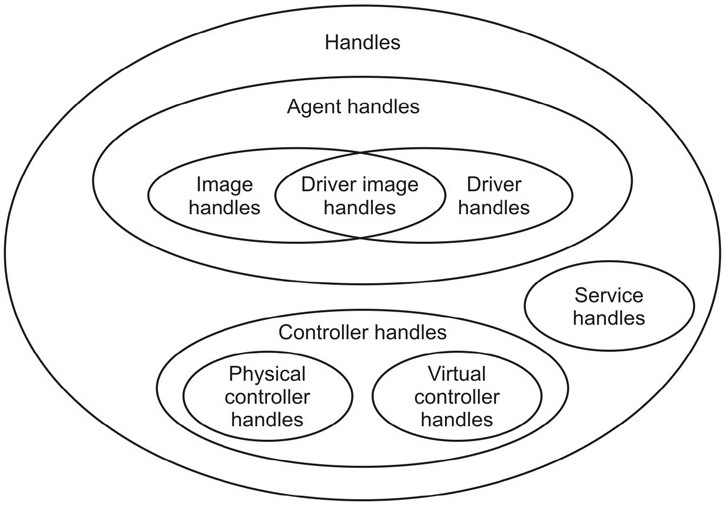
\includegraphics[width=0.7\textwidth]{uefi/handle_types}%
    \caption{Handle types (taken from \cite[Figure 3]{tianocore-edk2-driver-writer-s-guide})}%
    \label{fig:handle-types}%
\end{figure}

\cite{tianocore-edk2-driver-writer-s-guide} explains the categories of handles that are formed by the type of protocols that are grouped. \autoref{fig:handle-types} shows these categories.

\begin{description}
    \item[Image handles] are handles of \ac{UEFI} images loaded into memory, as they support the \hyperref[lst:loaded-image-protocol]{Loaded Image Protocol}, giving access to information about the image in memory. This includes the image's address, size, memory type, origin and optional load options.
    \item[Driver handles] are handles that group the \ac{UEFI} Driver Model related protocols (Driver Binding Protocol, the two Component Name Protocols and the two Driver Diagnostics Protocols)
    \item[Driver image handles] are \ac{UEFI} Driver Model related protocols installed onto images loaded in memory.
    \item[Agent handles] is a term used in the \ac{UEFI} Driver Model, they describe tracked consumers of other protocols.
    \item[Controller/Device handles] are interchangably used to refer to physical and virtual devices that offer \ac{I/O} abstraction protocols.
        Physical device handles support the Device Path Protocol for generic path/location information \cite[Section 10.2]{uefi-spec}.
    \item[Service handles] are used for generic hardware unrelated abstractions.
\end{description}

\TODO{\ac{I/O} abstractions}

\subsection{\acs{UEFI} Driver Model}

\cite[Section 2.5.2]{uefi-spec} describes the \acs{UEFI} Driver Model, it simplifies the design of device drivers by moving implementation of the device mangement and discovery into the firmware, leaving drivers with only the responsibility to offer interfaces for installation and removal.

We will focus on device drivers, these do not add any new device handles but instead offer protocol abstractions build upon already existing \ac{I/O} abstractions offered by bus drivers.
A driver following the \ac{UEFI} Driver Model is not allowed to interact with any hardware in its entry point and is instead required to install an instace of the Driver Binding Protocol on its own image handle.
The Loaded Image Protocol also offers a field where a driver can provide a function to unload itself.
It may also additionally install the confirguration or diagnostic related protocols.
Runtime drivers usually register a notification function that is triggered when an \ac{OS} loader calls \code{ExitBootServices}, this allows them to translate any allocated memory to their virtual addresses.

The firmware will try to connect device drivers to a controller by iterating over all instances of the Driver Binding Protocol in the handle database and calling the \code{Supported} function of the Driver Binding Protocol on a controller. The device driver then checks whether it supports the controller by for example looking for specific \ac{I/O} abstraction protocols, that it will want to laters use and further abstract.
If the driver supports the device the firmware will call the \code{Start} function of the Driver Binding Protocol to have the driver install its offered protocols on the controller handle.
This is done recursively as the newly installed device driver might now fullfill the requirements for another driver.
The firmware can also call the \code{Stop} of the Driver Binding Protocol function if it wants a driver to uninstall its protocol instance from a controller, an example for this would be another device driver wanting to exclusively manage a controller. This is done by tracking agents of protocols, in other words the drivers who consume a protocol.

\subsection{Systemtable}

The UEFI System Table is an important data structure, it provides access to system configuration information, generic boot and runtime services \cite[Section 3.3]{tianocore-edk2-driver-writer-s-guide}.
It also serves as the entrance in to the \ac{UEFI} environment, as a loaded images receives a only pointer to the system table as well as its image handle through its entry point. Although the Loaded Image Protocol provides and interface to hand optional load options to the image \cite{beyond-bios}.

\autoref{fig:uefi-system-table}


\TODO{during boot boot and runtime services are available}

\begin{figure}[htb]%
    \centering%
    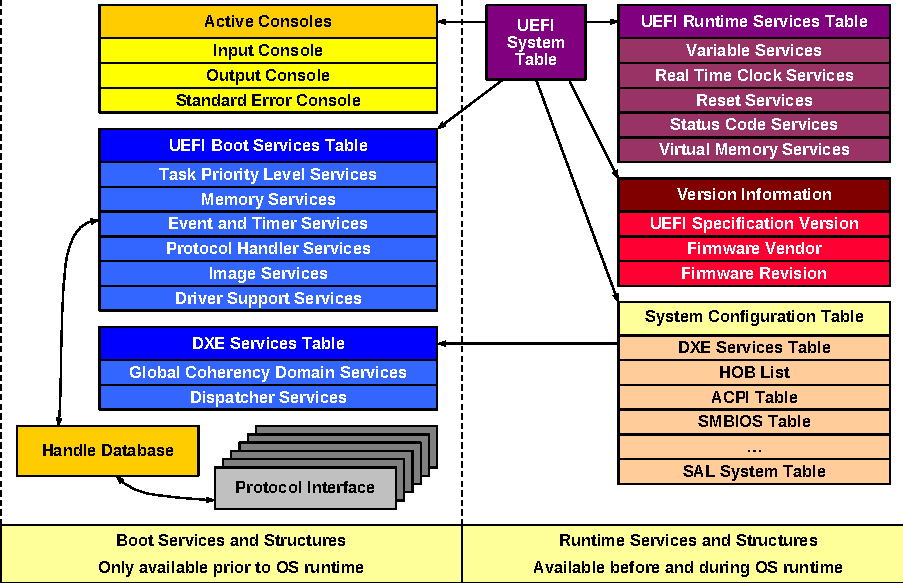
\includegraphics[width=0.8\textwidth]{uefi/uefi_system_table}%
    \caption{\ac{UEFI} System Table (taken from \cite[Vol 2, Figure 2-5]{pi-spec})}%
    \label{fig:uefi-system-table}%
\end{figure}


\subsubsection{Boot Services}

\ac{UEFI} applcations must use boot services functions to access devices and allocate memory. They are available until an \ac{OS} loader takes control over the system via a call to the boot service \code{ExitBootServices()}, from which on only runtime services are available. \cite[Section 7]{uefi-spec} splits the boot services into five categories:

\begin{description}
    \item [Event, Timer, and Task Priority Services] used to create, close, signal, wait for and check events. Setting timers and raising or restoring task priority levels.
    \item [Memory Allocation Services] to allocate and free pools or whole pages of memory, as well as retrieve the \ac{UEFI} managed memory map.
    \item [Protocol Handler Services] used to install, uninstall and retrieve protocol instance as well as abstractions related to the \ac{UEFI} Driver Model.
    \item [Image Services] to load, unload and start images. Images can also use these to transfer execution back to the firmware or with \code{ExitBootServices()} assume control over the system
    \item [Miscellaneous Services] offer basic memory manipulation, checksum calculation, watchdog timers and monotonic counters.
\end{description}

\subsubsection{Runtime Services}

\TODO{me}

\begin{description}
    \item [Variable Services] used to query, get and set \hyperref[sec:uefi-pi:uefi:variables]{variables}.
    \item [Time Services] used to get and set time as well as a system wakeup timer.
    \item [Virtual Memory Services] relate to enabling virtual memory and translating memory addresses.
    \item [Image Services] to load, unload and start images. Images can also use these to transfer execution back to the firmware or with \code{ExitBootServices()} assume control over the system
    \item [Miscellaneous Runtime Services] offer system reset, a monotonic counter and capsule services. Capsules allow the \ac{OS} to pass data to the firmware, this includes firmware managment related data.
\end{description}

\subsection{Variables}
\label{sec:uefi-pi:uefi:variables}

\ac{UEFI} variables are key/value pairs used to store arbitrary data passed between the \ac{UEFI} firmware and \ac{UEFI} applications.
The data type has to be known beforehand and as such is specified for variables defined in \ac{UEFI}.
The Storage implementation is not specified by \ac{UEFI}, but it must support non\-/volatility, to retain after reboots, or temper resistance if demanded.
Variables are defined by a vendor \ac{GUID}, a name and attributes.
Attributes include their scope (boot, runtime, non-volatile), whether writes require authentication or result in appending data instead of overwriting \cite[Section 8.2]{uefi-spec}.
Architecturally defined \ac{UEFI} variables are called Globally Defined Variables where the vendor \ac{GUID} has the value \code{EFI\_GLOBAL\_VARIABLE} \cite[Section 3.3]{uefi-spec}.

\subsection{Boot Manager}
\label{sec:uefi-pi:uefi:boot-manager}

The \ac{UEFI} boot manager is a firmware component executed after the platform is completely initialized, it decides which \ac{UEFI} drivers or applcations are loaded and when.
The boot behavior is configured through architecturally defined \ac{NVRAM} global variables\cite[Section 3.1]{uefi-spec}.
Each load option entry for a driver or application resides in a variable following the naming scheme of \code{Driver\#\#\#\#} or \code{Boot\#\#\#\#} respectively. Where \code{\#} stands for a hexadecimal digit forming a 4 digit number, requiring leading zeros.
If a firmware implementation allows for the creation of new load options they can then be added to the ordered lists \code{DriverOrder} and \code{BootOrder}, they reference load options and dictate the order in which they are processed.
Driver load options are processed before the boot load options, there also exists the \code{BootNext} variable to override the boot options once.
A general depiction of the \ac{UEFI} boot flow can be seen in \autoref{fig:uefi-boot-sequence}.
Implementations usually allow for an interactive menu, where users can modify the order or boot entries manually \cite[Section 3.1.1]{uefi-spec}.
Boot options are generally first attempted to be loaded through the \code{LoadImage} boot service.
If the device path of a boot option only points to a device instead to the file on a device, it attempts to load a default boot application with the \hyperref[lst:simple-file-system-protocol]{Simple File System Protocol}\cite[Section 3.1.2]{uefi-spec}, for x64 it uses the default path \code{\textbackslash EFI\textbackslash BOOT\textbackslash BOOTX64.EFI} \cite[Section 3.5]{uefi-spec}.

\begin{figure}[htb]%
    \centering%
    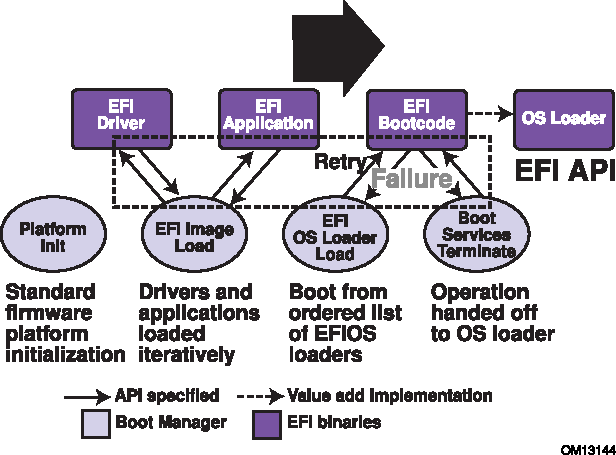
\includegraphics[width=0.8\textwidth]{uefi/uefi_boot_sequence}%
    \caption{Booting Sequence (taken from \cite[Figure 2-1]{uefi-spec})}%
    \label{fig:uefi-boot-sequence}%
\end{figure}

% !TeX root = ../../thesis.tex

\section{\acf{PI}}

\subsection{\acs{PI} Architecture Firmware Phases}

The \ac{PI} Architecture defines distinct phases.
focus will be on dxe and transient system load
\autoref{fig:pi-phases}



\begin{figure}[htb]%
    \centering%
    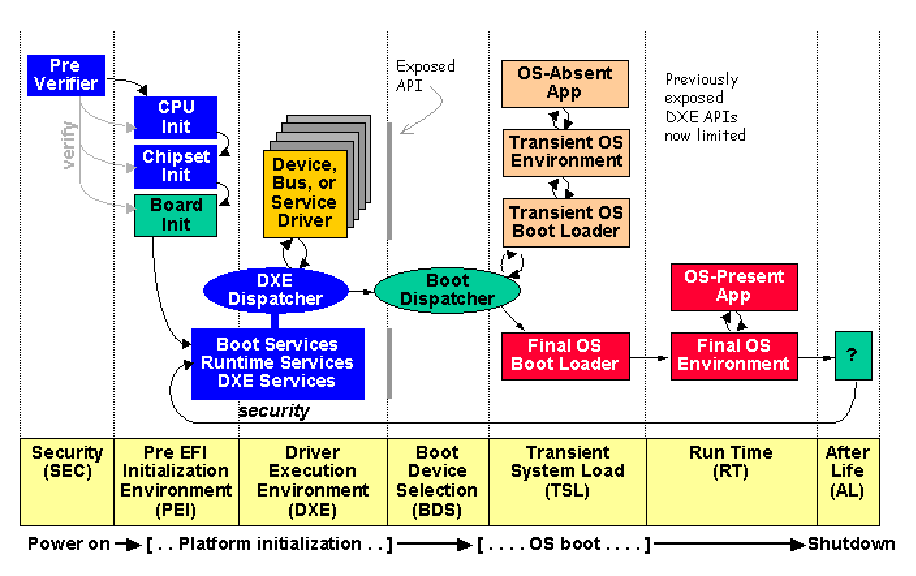
\includegraphics[width=\textwidth]{pi_boot_sequence}%
    \caption{\ac{PI} Architecture Firmware Phases \cite[Figure 2-1]{pi-spec}}%
    \label{fig:pi-phases}%
\end{figure}


\begin{enumerate}
    \item{\acf{SEC}}
    % % Since the CPU doesn't know about UEFI or BIOS the initial step is exactly the same, it starts in 16-bit real mode and fetches it's first instruction from `CS = 0xF000` and `IP = 0xFFF0` but instead of shifting `CS` left by four bits and adding `IP`, the `CS` base register is initialized to `0xFFFF'0000`. So the first instruction is fetched from the physical address `0xFFFF'FFF0` (`0xFFFF'0000 + 0xFFF0`). The CS base address remains at this initial value until the CS selector register is loaded by software (e.g. far jump or call instruction)

    % \begin{itemize}
    %     \item Populates Reset Vector Data structure
    %     \item Saves Built-in self-test (BIST) status
    %     \item Enables protected mode (16 bit -> 32 bit)
    %     \item Configures temporary RAM (not only limited in processor cache) by using MTRR to configure CAR.
    % \end{itemize}


    The \ac{SEC} phase is the first phase performed during platform initialization. Under its responsibilities fall handling all platform restart events, setting up temporary memory and establishing the system's root of trust. It serves as the foundation for all secure operations on which inductive security designs rely to build a chain of trust by having a module verify the integrity of its subsequent module. For this the \ac{SEC} phase may verify the integrity of the \ac{PEI} foundation before transfering execution to it. When it transfers execution, it also passes information about the current state of the system, including location and size of the temporary stack, \ac{RAM}, and \ac{BFV}. It can also optionally pass protocols for the \ac{PEI} phase to use.

    \item{\acf{PEI}}

    Configures a system meeting the minimum prerequisites for the Driver Execution (DXE) phase, which is generally a linear array of RAM large enough for successful execution.

    PEI provides a framework allowing vendors to supply initialization modules for each functionally distinct piece of system hardware which must be initialized before the DXE phase.

    PEI design goals of the PI architecture:
    \begin{itemize}
        \item Maintenance of the chain of trust, includes protection and authorization of PEI modules
        \item Provide a core PEI module
        \item Independent developement of intialization modules
    \end{itemize}
    The PEI phase consists of the PEI Foundation core and specialized plug-ins known as Pre-EFI Initialization Modules (PEIMs).

    Since the PEI phase is very early in the boot process it can't assume reasonable amounts of RAM so the features are limited:
    \begin{itemize}
        \item Locating, validating and dispatching PEIMs
        \item Communication between PEIMs
        \item Providing Hand-Off Data for DXE phase
        \item Initializing some permanent memory complement
        \item Describing the memory in Hand-Off Blocks (HOBs)
        \item Describing the firmware volume locations in HOBs
        \item Passing control into the Driver Execution Environment (DXE) phase
        \item Discover boot mode and possibly resume from sleep state
    \end{itemize}
    PEI Service Table visible to all PEIMs in the system, a pointer to this table is passed as an argument via the PEIM entry point, it is also part of each PEIM-to-PEIM Interface (PPI).


    % | Service                  | Description                                                                                                                                 |
    % | ------------------------ | ------------------------------------------------------------------------------------------------------------------------------------------- |
    % | PPI Services             | Manages PPIs to facilitate intermodule calls between PEIMs. Interfaces are installed and tracked on a database maintained in temporary RAM. |
    % | Boot Mode Services       | Manages the boot mode (S3, S5, normal boot, diagnostics, etc.) of the system                                                                |
    % | HOB Services             | Creates data structures called Hand-Off Blocks (HOBs) that are used to pass information to the next phase of the PI Architecture.           |
    % | Firmware Volume Services | Finds PEIMs and other firmware files in the firmware volumes                                                                                |
    % | PEI Memory Services      | Provides a collection of memory management services for use both before and after permanent memory has been discovered                      |
    % | Status Code Services     | Provides common progress and error code reporting services (for example, port 080h or a serial port for simple text output for debug).      |
    % | Reset Services           | Provides a common means by which to initiate a warm or cold restart of the system.                                                          |

    % #### PEI Foundation/Core

    PEI Foundation code is portable across all platforms of a given instruction-set. The set of exposed services is the same across different microarchitextures and allows PEIMs to be written in C.

    - Dispatches PEIMs
    - Maintains boot mode
    - Initializes permanent memory
    - Invokes DXE loader

    % #### PEI Dispatcher

    The PEI Dispatcher evaluates dependencies of PEIMs in the firmware volume, these dependencies are PPIs. The Dispatcher holds internal state machines to check dependencies of PEIMs, it starts executing PEIMs whose dependencies are statisfied to build up dependencies of other PEIMs, this is done until the dispatcher cannot invoke any more PEIMs. Then the DXE Initial Program Loader (IPL) PPI is invoked to pass control to the DXE phase.

    % #### Pre-EFI Initialization Modules (PEIMs)
    PEIMs are specialized drivers that personalize the PEI Foundation to the platform. They are analogus to DXE driver and generally correspond to the components being initialized. It is strongly recommended that PEIMS do only the minimum necessary work to initialize the system to a state that meets the prerequisites of the DXE phase. PEIMs reside in firmware volumes (FVs).

    % #### PEIM-to-PEIM Interfaces (PPIs)
    PEIMs communicate with each other using a structure called PPI. A PPI is a GUID pointer pair. The GUID is used to identifiy a certain service and the pointer provides access to data structures and services of the PPI.

    % There are two kinds of PPIs:
    % - Architectural PPIs
    % - Additional PPIs

    An architectural PPI is described in the PEI Core Interface Specification (CIS) and the GUID is known to the PEI Foundation. They typically provide a common interface to the PEI Foundation to a service with platform specific implementation.

    An additional PPI is important for interoperability but isn't required by the PEI Foundation, they can be classified as mandatory or optional.


    \begin{itemize}
        \item init permanent memory
        \item describe memory in \acp{HOB}
        \item describe \ac{FV} in \acp{HOB}
        \item pass control to \ac{DXE}
    \end{itemize}

    crisis recovery (what is this?)
    resuming from S3 sleep state
    linear array of RAM
    \ac{PEIM} provides a framework to allow vendors to supply separate initialization modules for
    each functionally distinct piece of system hardware that must be initialized prior to the DXE phase \cite{pi-spec}

    % design goals
    maintenance of chain of trust, protection against unauthorized updates to the PEI phase or modules
    authentication of the PEI Foundation and its modules
    provide core PEI module (PEI foundation) processor architecture independent, supports add-in moudles from vendors for processors, chipsets, RAM

    % what it does
    Locating, validating, and dispatching PEIMs
    Facilitating communication between PEIMs
    Providing handoff data to subsequent phases

    \item{\acf{DXE}}


    % - DXE Foundation/Core
    % - DXE Dispatcher
    % - DXE Drivers

    % #### DXE Foundation

    The DXE Foundation produces a set of Boot, Runtime and DXE Services and exposes them through handle databases in the EFI System Table. It is designed to be completely portable, independent of processor, chipset and platform. The only dependent of the Hand-Off Blocks from the PEI phase, after these are processed the all prior phases can be unloaded.

    % #### DXE Dispatcher

    The DXE Dispatcher discovers DXE drivers within the Firmware Volume (FV) and executes them in the correct order, respecting their dependencies towards each other. The Firmware Volume file format allows the DXE driver images to be packaged with expressions about their dependencies. Since the DXE Drivers are PE/COFF images the dispatcher comes with an apropriate loader to load and execute the image format.

    % #### DXE Drivers

    % - Drivers that execute very early in the DXE phase
    % - Drivers that comply with the UEFI Driver Model

    The DXE Drivers are responsible for initializing the processor, chipset,
    and platform components as well as providing software abstractions for console and
    boot devices in the form of services.

    dxe core/foundation
    platform independent
    is implementation of UEFI
    UEFI Boot Services
    UEFI Runtime Services
    DXE Services

    dxe dispatcher
    discover drivers stored in firmware volumes and execute in proper order
    apriori file optionally in FV or depex of driver
    after dispatching all drivers in the dispatch queue hands control over to BDS

    dxe drivers
    init processor, chipset and platform
    produce arichtectural protocols and \ac{I/O} abstractions for consoles and boot devices

    % responsibilities
    initializing the processor, chipset, and platform components
    providing software abstractions for system services, console devices, and boot devices.

    \item{\acf{BDS}}
    The DXE Foundation will hand control to the BDS Architectural Protocol after all of the DXE drivers whose dependencies have been satisfied have been loaded and executed by the DXE Dispatcher.

    % - Initializing console devices based on the ConIn, ConOut, and StdErr environment variables
    % - Loading device drivers listed in the DriverOrder environment variables
    % - Attempting to load and execute boot selections list from the BootOrder environment variables

    During the BDS phase new Firmware Volumes (FV) might be discovered and control is once again handed to the DXE Dispatcher to load drivers found on these additional volumes.


    DXE arichtectural protocol
    one function entry
    platform boot

    attempts to connect boot devices required to load the os
    discovers volumes containing new drivers
    calls DXE dispatcher
    doesnt return when successfully booting OS

    UEFI itself only specifies the NVRAM variables used in selecting boot options
    leaves the implementation of the menu system as value added implementation space \cite{uefi-spec}

    \cite{pi-spec}

    \begin{itemize}
        \item Initializing console devices
        \item Loading device drivers
        \item Attempting to load and execute boot selections
    \end{itemize}

    \item{\acf{TSL}}

    The Transient System Load (TSL) is primarily the OS vendor provided boot loader. Both the TSL and the Runtime Services (RT) phases may allow access to persistent content, via UEFI drivers and UEFI applications. Drivers in this category include PCI Option ROMs.

    This phase ends when an OS boot loader calls 'ExitBootServices()'.

    boot and runtime services/driver
    bootloader
    \cite[Section 13.3]{uefi-spec}
    \cite[Section 3.5.1.1]{uefi-spec}

    ExitBootServices()

    \item{\acf{RT}}
    Boot service drivers have been unloaded and only runtime services are accessible.


    runtime services/driver

    \item{\acf{AL}}
    The After Life (AL) phase consists of persistent UEFI drivers used for storing the state of the system during the OS orderly shutdown, sleep, hibernate or restart processes.

    hibernation
    sleep

\end{enumerate}

\subsection{\acs{UEFI}/\acs{PI} Firmware Images}

Firmware Images are stored in Flash Devices (FD), a Firmware Volume (FV) serves as file level interface. Usually multiple FVs are present in a single FD but a signle FV can also be distributed via multiple FDs.
A FV is formatted with a binary file system, typically with Firmware File System (FFS).

In a FFS modules are stored as files, they can be executed at the fixed address from Read Only Memory (ROM) or through relocation in loaded memory. Within a file are multiple sections which then contain the "leaf" images. These are for example PE32 images.

% https://edk2-docs.gitbook.io/edk-ii-build-specification/2_design_discussion/22_uefipi_firmware_images
\cite[Vol. 3, Section 2.1]{pi-spec}

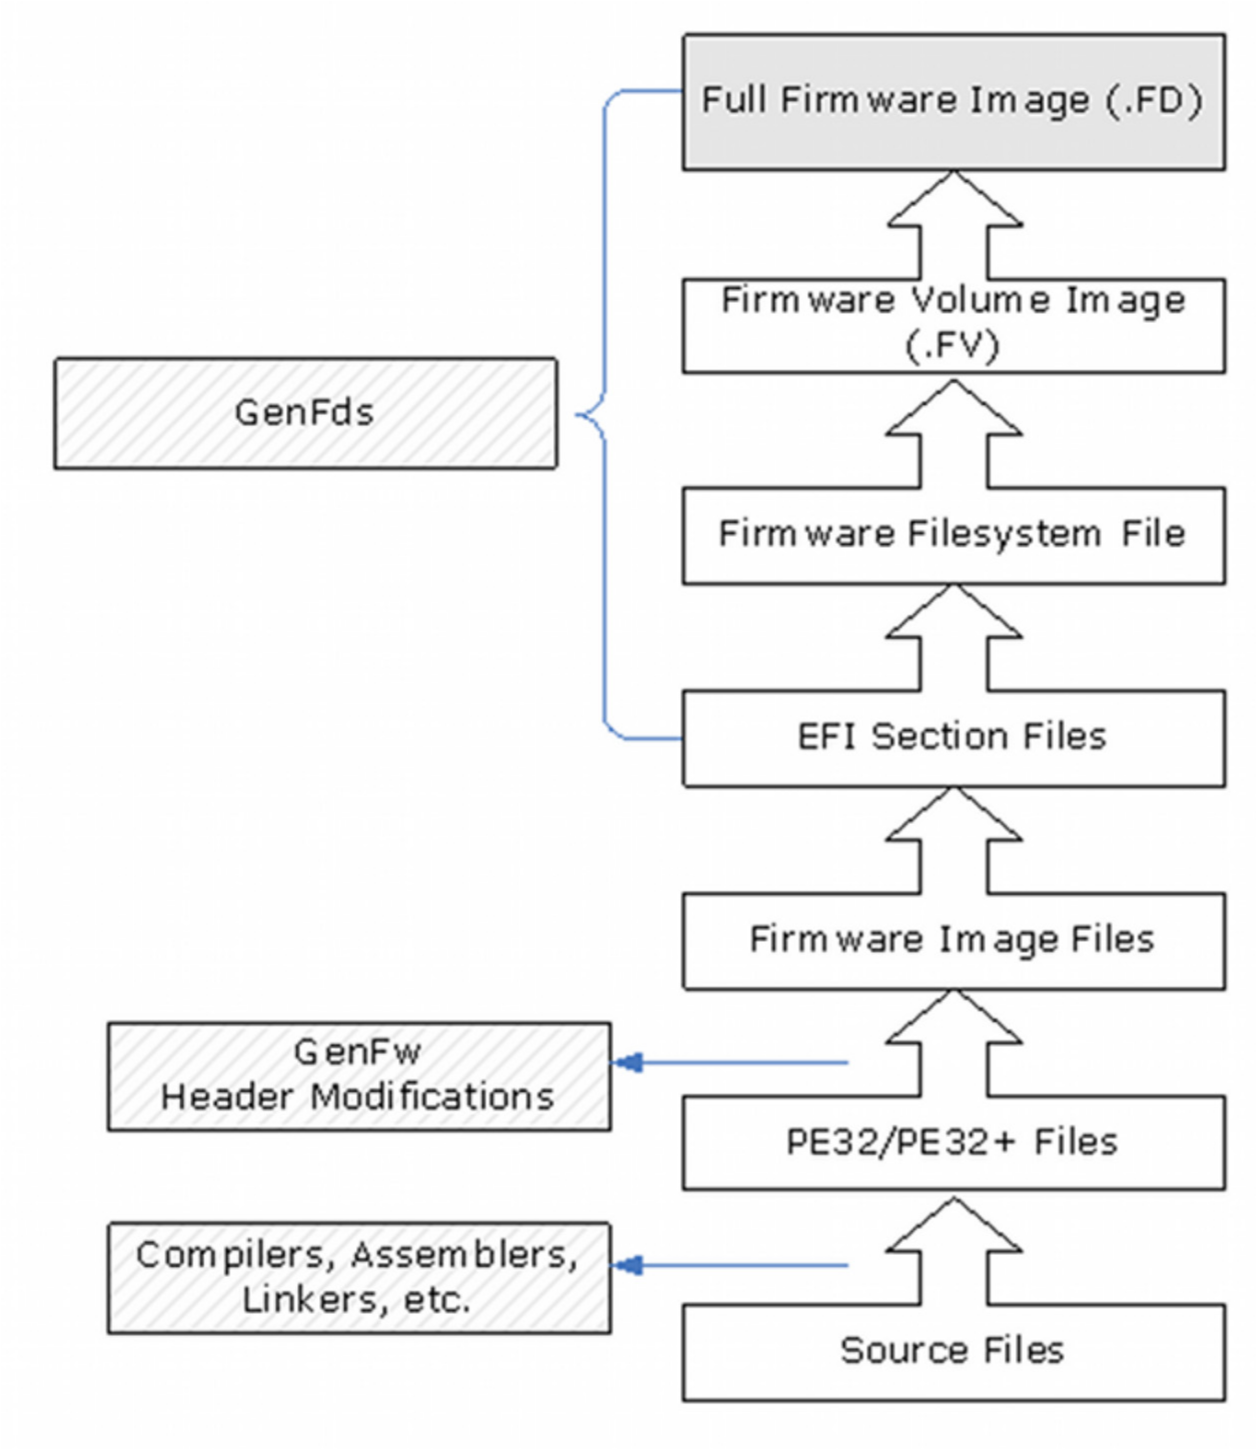
\includegraphics[width=\textwidth]{flash_device}
\ac{FD}
persistent
physical device
contains firmware code and/or data
typically flash
may be divided into smaller pieces to form multiple logical firmware devices
multiple physical firmware devices may be aggregated into one larger logical firmware device

\acf{FV}
logical device
organized into a file system
attributes such as
- size
- formatting
- read/write access

\acf{FFS}
organization of files and free space
no dierectory hierarchy
all files flat in root dir
parsing requires walking for beginning to end

firmware files
types
% PEI_CORE
% PEIM
% DXE_CORE
% DRIVER
% FIRMWARE_VOLUME_IMAGE
% FREEFORM

some file types are sub-divided in file sections

file sections can be either
encapsulation or leaf
leaf sections such as
PE32
% DXE_DEPEX
% PEI_DEPEX
RAW
VERSION
TE

dxe drivers files
contain one PE32 executable section
may contain version section
may contain dxe depex section

freeform files
can contain any combination of sections

PEI phase Service Table
FfsFindNextFile, FfsFindFileByName and FfsGetFileInfo

DXE phase
% EFI_FIRMWARE_VOLUME2_PROTOCOL

depex

\cite{tianocore-edk2-build-spec}

% !TeX root = ../../thesis.tex

\subsection{Security}
\label{sec:uefi-pi:pi:security}

The \ac{PI} specification defines \acp{PPI} and \ac{DXE} protocols which can be used to validate images when loading them.
During the \ac{PEI} phase, the \emph{\ac{PEI} Guided Section Extraction \ac{PPI}} can be used to authenticate file sections, while the \emph{Security \ac{PPI}} implements the policy response to the authentication result.
The \ac{DXE} phase has counter parts in the form of the \emph{Guided Section Extraction Protocol} and the \emph{Security Architectural Protocol}.
The policy response may be the locking of flash upon authentication failure or attestation logging \cite[Vol. 2, Section 12.9.1]{pi-spec}.
It also has the architectural protocol \emph{Security2 Architectural Protocol}, which implements Secure Boot validation, \ac{TCG} measured boot, and User Identity policy for image loading.
The implementation of the boot service \code{LoadImage()} has to use these protocols in accordance to the rules defined in \cite[Vol. 2, Section 12.9.2]{pi-spec}.
The Security2 protocol is invoked on every loaded image, with the Security protocol being invoked afterwards on images loaded through the Firmware Volume Protocol.
When the Security2 protocol is not installed it uses the Security protocol regardless of the image's origin.

\subsubsection{Hardware Validated Boot}

Secure Boot relies on the firmware as its root of trust.
Hardware validated boot is able to shift the root of trust out of the firmware image into a smaller part in the hardware, in hopes to reduce the size of the attack vector.
This part performs validation of the \ac{IBB} before handing over execution to the firmware image \cite{tianocore-understanding-uefi-secure-boot-chain}.

\subsubsection{Firmware Protection}

The \ac{PI} specification defines an \emph{End of \acs{DXE} Event}, which indicates the introduction of third party software execution to the platform.
Up until this point it is assumed that the entire system software is under the control of the platform manufacturer.
Drivers may react to this event by locking critical system resources, using the \ac{SMM} related services \cite[Vol. 2, 5.1.2.1]{pi-spec}.
The \ac{SMM} is a secure execution environment, achieved by isolation from the rest of the system, through the \ac{CPU} \cite[Vol. 4, Section 1.3]{pi-spec}.
The \ac{PI} reference implementation also makes use of this event to lock the device that stores the firmware image \cite{tianocore-edk2-fmpdxe}.


% !TeX root = ../thesis.tex

\subsection{Security}

others not discussed further
user identification

PEI
GuidedSection Extraction


\subsubsection{Secure Boot}
% https://learn.microsoft.com/en-us/windows/security/information-protection/secure-the-windows-10-boot-process
% https://edk2-docs.gitbook.io/understanding-the-uefi-secure-boot-chain/secure_boot_chain_in_uefi/uefi_secure_boot
% https://papers.vx-underground.org/papers/Other/Advanced%20Malware/UEFI%20Secure%20Boot%20in%20Modern%20Computer%20Security%20Solutions.pdf

\cite{tianocore-understanding-uefi-secure-boot-chain}

% workings of secure boot
driver signing
executables may be located on un-secured media
system provider can authenticate either origin or integrity

digital signature
data to sign
public/private key pair used to verify integrity

% how it is signed

embedded within PE file
calculating the pe image hash
- hashing the pe header, omitting the file's checksum and the Certificate Table entry in Optional Header Data Directories
- sorting and hasing pe sections
omitting attribute certifacte table and hash remaining data

\cite{microsoft-pe-signature-format}


% key and hash storage

% how, when and where is it verified

guarantees only valid 3rd party firmware code can run in OEM firmware environment
UEFI Secure Boot assumes the system firmware is a trusted entity
any 3rd party firmware code is not trusted
including bootloader/osloader, PCI option ROMs, UEFI shell tool

two parts
verification of the boot image and verification of updates to the image security database
\cite{tianocore-understanding-uefi-secure-boot-chain}

Secure Boot uses the content of the SPI flash memory as its root of trust\cite{lojax}


\subsubsection{Firmware Protection}

% https://eclypsium.com/2019/10/23/protecting-system-firmware-storage/

DXE SMM Ready to Lock Vol4

Capsule Architectural Protocol

provides
CapsuleUpdate()
QueryCapsuleCapabilities()
of the runtime services table

flash device security

\subsubsection{TPM measurements}
% https://tianocore-docs.github.io/edk2-TrustedBootChain/release-1.00/
% https://tianocore-docs.github.io/edk2-TrustedBootChain/release-1.00/3_TCG_Trusted_Boot_Chain_in_EDKII.html
% https://tianocore-docs.github.io/edk2-TrustedBootChain/release-1.00/6_Checklist_for_Platform_Developers.html
% https://learn.microsoft.com/en-us/windows/security/information-protection/tpm/tpm-fundamentals
% https://learn.microsoft.com/en-us/windows/security/information-protection/tpm/trusted-platform-module-overview
% what is TPM
A \acf{TPM} is a system component which enables trust in computing platforms
helps verify if the Trusted Computing Base has been compromised
securely storing passwords, certificates and encryption keys in separate state to host
only communicating through a well defined interface.
store platform measurements that help ensure that the platform remains trustworthy
authentication
attestation
hardware and software implementations
software special mode shielding TPM resources from normal execution
\cite{tcg-tpm-summary}
\cite{tcg-tpm-library-part1-architecture}

% what is done with the measurements
% https://learn.microsoft.com/en-us/windows/security/information-protection/bitlocker/bitlocker-overview
how are they used
works with bitlocker to protect user data
ensure computer has not been tampered with while offline

% what is measured
statically configured, unchangeable data
not dynamic and changeable across the boot,
\cite{tianocore-trusted-boot-chain}

\begin{tabular}{ |c||c|  }
    \hline
    \acs{PCR} Index & \acs{PCR} Usage                                                                                          \\
    \hline
    \hline
    0               & SRTM, BIOS, Host Platform Extensions, Embedded Option ROMs and PI Drivers                                \\
    \hline
    1               & Host Platform Configuration                                                                              \\
    \hline
    2               & UEFI driver and application Code                                                                         \\
    \hline
    3               & UEFI driver and application Configuration and Data                                                       \\
    \hline
    4               & UEFI Boot Manager Code (usually the MBR) and Boot Attempts                                               \\
    \hline
    5               & Boot Manager Code Configuration and Data (for use by the Boot Manager Code) and \ac{GPT}/Partition Table \\
    \hline
    6               & Host Platform Manufacturer Specific                                                                      \\
    \hline
    7               & Secure Boot Policy                                                                                       \\
    \hline
    8               & First \ac{NTFS} boot sector (volume boot record)                                                         \\
    \hline
    9               & Remaining \ac{NTFS} boot sectors (volume boot record)                                                    \\
    \hline
    10              & Boot Manager                                                                                             \\
    \hline
    11              & BitLocker Access Control                                                                                 \\
    \hline
\end{tabular}
\cite{tcg-pc-client-platform-firmware-profile-spec, winwos-internals-6-part2}

% https://tianocore-docs.github.io/edk2-TrustedBootChain/release-1.00/media/image2.png

% https://tianocore-docs.github.io/edk2-TrustedBootChain/release-1.00/3_TCG_Trusted_Boot_Chain_in_EDKII.html
% Table 2 PCR usage (simple rules)

% https://tianocore-docs.github.io/edk2-TrustedBootChain/release-1.00/media/image3.png

% when is it measured
\cite{tianocore-trusted-boot-chain}

% where is it measured
\ac{TCG}2 Protocol
Trusted Computing Group 2 (TCG2) Protocol \cite[6.7.3]{tcg-efi-protocol-spec}

% secret storage, seal and unseal


\section{\acs{EDK} II}
build system
at least mention that local gcc is used, relevant for porting and headers

BaseTools package process files compiled by third party tools, as well as text and Unicode files in order to create UEFI or PI compliant binary image files
\cite{tianocore-edk2}